
\documentclass[a4paper,12pt]{article}

% Pakete
\usepackage[utf8]{inputenc}     % UTF-8 Kodierung
\usepackage[T1]{fontenc}        % Font Encoding
\usepackage{graphicx}           % Bilder einfügen
\usepackage{caption}            % Bildbeschriftungen
\usepackage{geometry}           % Seitenränder
\usepackage{hyperref}           % Hyperlinks
\usepackage{float}              % [H] Position für Bilder

% Seitenlayout
\geometry{
    top=20mm,
    bottom=20mm,
    left=20mm,
    right=20mm
}

% Titel
\title{Aufgabenblatt 1: Visualisierung des Auto Datensatzes}
\author{Tim Lukas}
\date{\today}

\begin{document}

\maketitle

% ===========================
\section{Visualisierung 1}
\begin{figure}[H]
    \centering
    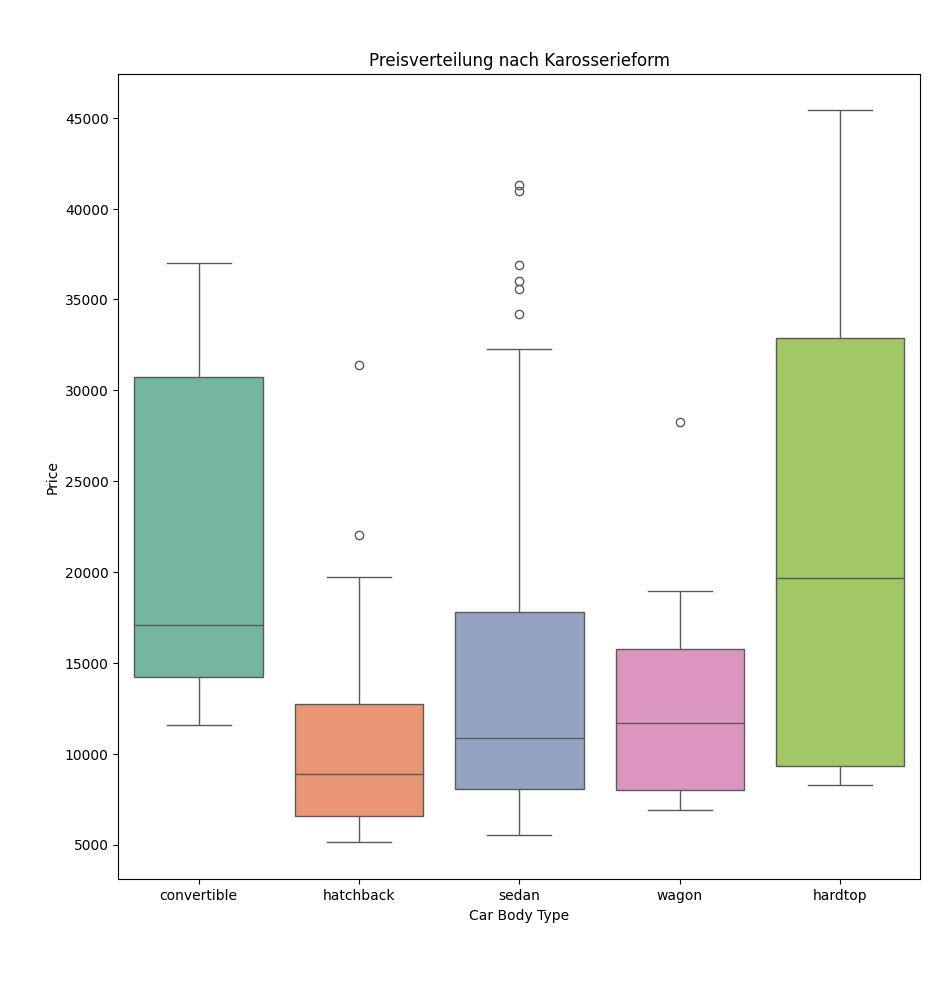
\includegraphics[width=0.8\textwidth]{../images/preisverteilung_nach_karrosserie.png} % Pfad zur Datei anpassen
    \caption{Preisverteilung nach Karosserieform}
    \label{fig:vis1}
\end{figure}

\subsection*{Beschreibung Visualisierung 1}
Diese Visualisierung zeigt das Verhältnis zwischen Preis und Karosserieform.

% ===========================
\section{Visualisierung 2}
\begin{figure}[H]
    \centering
    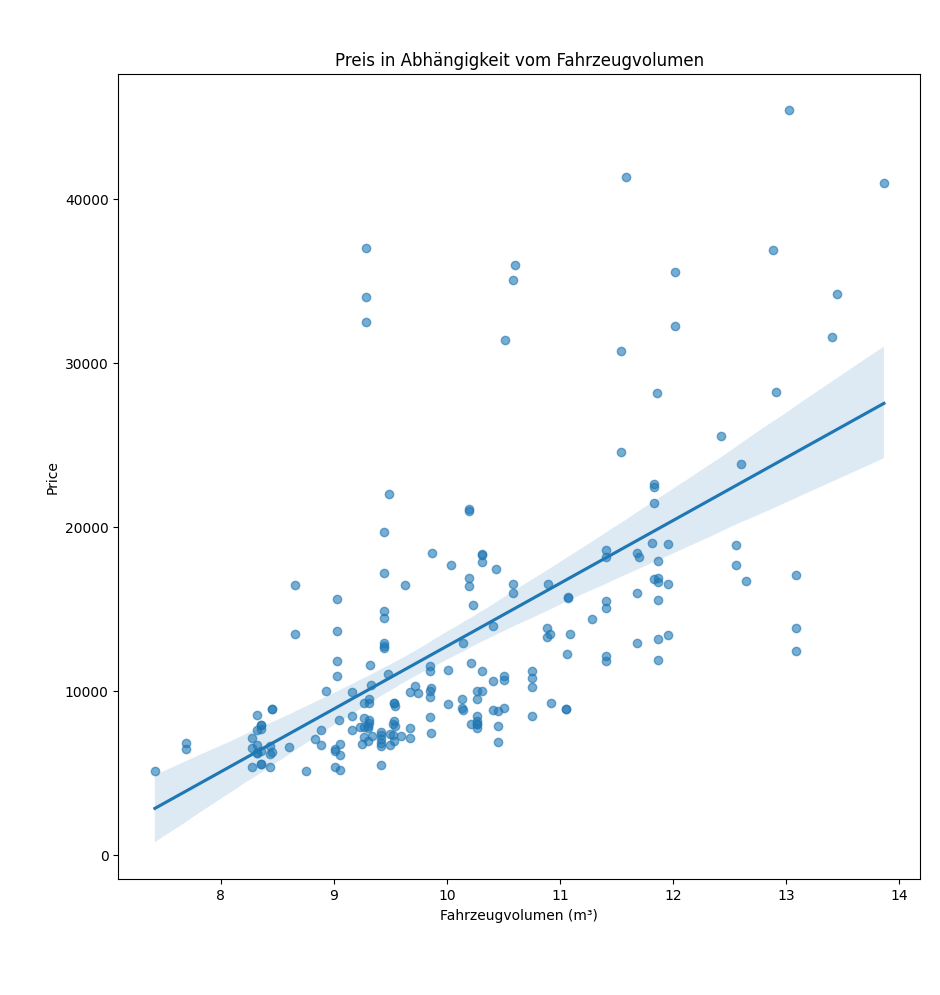
\includegraphics[width=0.8\textwidth]{../images/preis_nach_fahrzeugvolumen.png} % Pfad zur Datei anpassen
    \caption{Preis nach Fahrzeugvolumen}
    \label{fig:vis2}
\end{figure}

\subsection*{Beschreibung Visualisierung 2}
Die zweite Visualisierung bildet den Preis in Abhängigkeit vom Fahrzeugvolumen ab, dafür wurde das
Fahrzeugvolumen mit folgender Formel berechnet: 


% ===========================
\section{Visualisierung 3}
\begin{figure}[H]
    \centering
    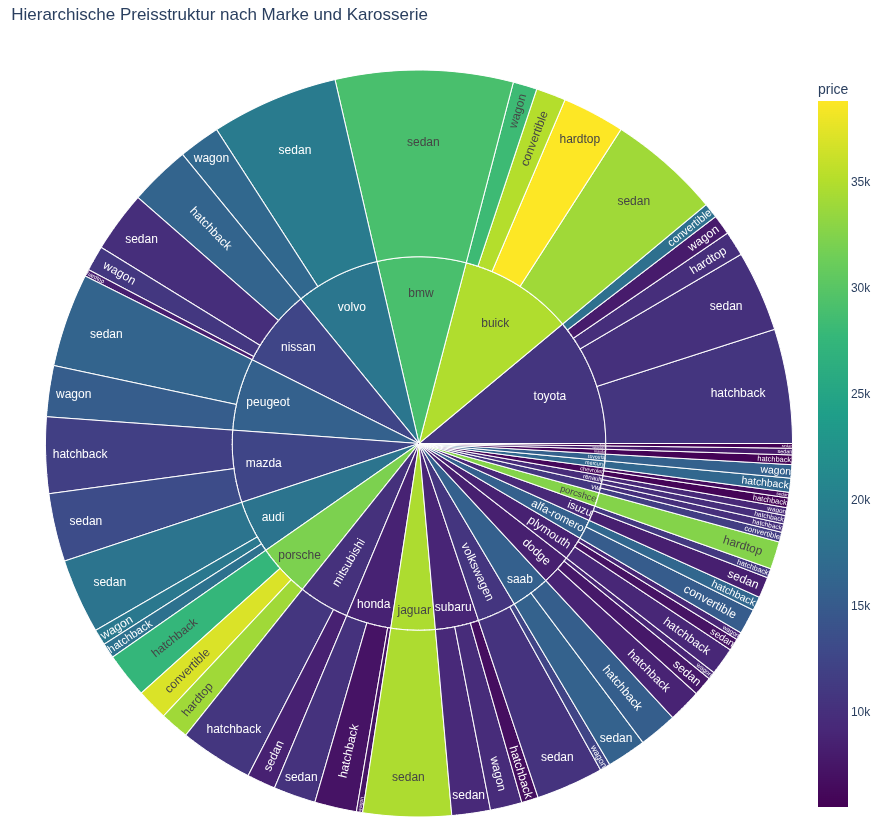
\includegraphics[width=0.8\textwidth]{../images/preisstruktur_nach_marke_karosserie.png} % Pfad zur Datei anpassen
    \caption{Preisstruktur nach Marke und Karosserie}
    \label{fig:vis3}
\end{figure}

\subsection*{Beschreibung Visualisierung 3}
Die dritte Viusalisierung zeigt die Preisstruktur der Fahrzeuge nach Marke und Karosserie an.


% ===========================
\section{Verwendete Tools}
Für die Erstellung der Visualisierungen wurden folgende Python-Tools verwendet:

\begin{itemize}
    \item \textbf{pandas}: Datenmanipulation und Einlesen von CSV-Dateien.
      Mit \texttt{pandas} konnten die Spalten ausgewählt, in numerische Werte konvertiert
      und neue Features wie das Fahrzeugvolumen berechnet werden.
    \item \textbf{matplotlib}: Grundlegende Visualisierung.
      Dient zum Erstellen von Scatterplots, Boxplots, 3D-Plots und zur Anpassung von Achsen, Titeln und Layouts.
    \item \textbf{seaborn}: Aufbauend auf \texttt{matplotlib} für statistische Visualisierungen.
      Genutzt für Scatterplots, Boxplots, Pairplots, Bubble-Charts, Heatmaps und die Anpassung von Farben, Transparenz und Layouts.
    \item \textbf{mpl\_toolkits.mplot3d}: Erweiterung von \textbf{matplotlib} für 3D-Darstellungen (z.B. 3D-Scatterplots).
    \item \textbf{plotly.express}: Erstellung interaktiver Visualisierungen (z.B. Sunburst-Diagramme).
      Unterstützt Zoom, Tooltipps und Farbkodierungen.
\end{itemize}


\end{document}
